\documentclass{atistandalonetask}
\usepackage{atistandard}
\begin{document}
  \begin{atiTask}[
    title = Expandieren die Maßstäbe?
  ]
    Wir betrachten ein gebundenes System, wie etwa das Planetensystem der Sonne oder ein \textsc{Bohr}sches Atom, welches in ein expandierendes Universum eingebettet ist und behandeln das \textsc{Kepler}-Problem mit der Annahme, dass die Masse eines der beiden Körper sehr viel größer sei als die des anderen.
    \begin{atiSubtasks}
      \item{ \locallabel{a}
        Zeigen Sie, dass der Einfluss der kosmischen Expansion durch einen \enquote{kosmischen Beschleunigungsterm} in der \textsc{Newton}schen Bewegungsgleichung gemäß
        \[
          \timeSecondDerivative{\vector{r}} - \frac{\timeSecondDerivative{a}}{a} \vector{r} = -\frac{GM}{r^2}\frac{\vector{r}}{r}
        \]
        berücksichtigt werden kann.
        Darin bedeutet $M$ die Zentralmasse, und der radiale Abstand $r$ der beiden Himmelskörper unterliegt dem \textsc{Hubble}-Gesetz.
        \[
          \timeDerivative{\vector{r}} = H r = \frac{\timeDerivative{a}}{a} \vector{r}
        \]
        Gilt auch unter den neuen Bedingungen Drehimpulserhaltung?
      }
      \item{ \locallabel{b}
        Diskutieren Sie diese Bewegungsgleichung anhand ihres effektiven Potentials.
        \begin{atiSubsubtasks}
          \item{
            Nehmen Sie realistischerweise an, dass die zeitabhängige Größe $\frac{a''}{a}$ für die Dauer eines Planetenumlaufs um die Sonne als konstant betrachtet werden kann.
            Drücken Sie diese Grüße durch die heutigen Werte von \textsc{Hubble}- und Beschleunigungs-Parameter aus.
          }
          \item{
            Definieren Sie einen kritischen Radius $r_\mathrm{krit}$ aus der Bedingung, dass kosmische Beschleunigung und Beschleunigung durch Gravitations-Anziehung den gleichen Betrag haben und drücken Sie diesen durch die Zentralmasse und die Massendichte eines \textsc{Einstein-DeSitter}-Kosmos aus.
          }
          \item{
            Stellen Sie das effektive Potential für verschiedene Werte des Verhältnisses $\frac{r_0}{r_\mathrm{krit}}$ graphisch dar, worin $r_0$ der Radius der ungestörten \textsc{Kepler}-Bahn ist.
          }
        \end{atiSubsubtasks}
      }
      \item{ \locallabel{c}
        Berechnen Sie für die nachfolgend genannten Systeme in einem \textsc{Einstein-DeSitter}-Kosmos die beiden Beschleunigungsanteile in der Bewegungsgleichung sowie den kritischen Radius und entscheiden Sie, ob diese Systeme mit dem Universum expandieren.
        \begin{atiSubsubtasks}
          \item{
            Das Planetensystem der Sonne --- die Astronomische Einheit als Maßstab.
          }
          \item{
            Der Umlauf der Sonne um das galaktische Zentrum: $r_0=8.5\appendUnit{kpc}$, $v=220\appendUnit{km\cdot s^{-1}}$
          }
          \item{
            Die Bewegung einer Galaxie am Rand des Kerngebietes eines Galaxienhaufens: $r_0 = 250\appendUnit{kpc}$, $v = 800\appendUnit{km\cdot s^{-1}}$
          }
          \item{
            Die Bewegung eines Elektrons auf der ersten \textsc{Bohr}schen Bahn nach dem \textsc{Bohr}schen Atommodell --- der \textsc{Bohr}sche Radius als Maßstab.
          }
        \end{atiSubsubtasks}
      }
    \end{atiSubtasks}
  \end{atiTask}
  \begin{atiSolution}
    \begin{atiSubtaskSolutions}
      \item[\localref{a}]{
        Zunächst parametrisieren wir den flachen Raum durch Kugelkoordinaten.
        \[
          \function{Φ}{\setReal^+\times [0,π] \times [0,2π)}{\setReal^3}
          \separate
          Φ(χ,ϑ,φ) \define
          \begin{pmatrix}
            χ \sin ϑ \cos φ \\
            χ \sin ϑ \sin φ \\
            χ \cos ϑ
          \end{pmatrix}
        \]
        Wir beschreiben die Expansion unseres Raumes in Abhängigkeit der Zeit durch die glatte Skalierungsfunktion $a$.
        \[
          \function{a}{\setReal}{\setReal^+}
        \]
        Die Position $r(t)$ eines festen Ortspunktes $(χ,ϑ,φ)$ zur Zeit $t\in\setReal$ ändert sich damit wie folgt.
        \[
          \function{r}{\setReal}{\setReal^3}
          \separate
          r(t) \define a(t) Φ(χ,ϑ,φ)
        \]
        Durch Differenzieren erhalten wir nun die folgenden Gleichungen.
        \[
          r'(t) = a'(t) Φ(χ,ϑ,φ) = \frac{a'(t)}{a(t)} r(t)
        \]
        \[
          r''(t) = a''(t) Φ(χ,ϑ,φ) = \frac{a''(t)}{a(t)} r(t)
        \]
        Die Beschleunigung eines Massenpunktes ergibt sich nun nach dem zweiten \textsc{Newton}schen-Axiom aus der Summe der beiden Beschleunigungen.
        Demnach wurde gezeigt, dass der Effekt der kosmischen Expansion durch die folgende Gleichung berücksichtigt werden kann.
        \[
          r'' = \frac{a''}{a}r - \frac{GM}{\norm{r}^3}r
        \]
        Um die Drehimpulsbilanz zu erhalten, bilden wir das linksseitige Kreuzprodukt mit $r$ und integrieren die erhaltene Gleichung.
        \[
          \crossProduct{r}{r''} = L' = \frac{a''}{a}\crossProduct{r}{r} - \frac{GM}{\norm{r}^3} \crossProduct{r}{r} = 0
        \]
        \[
          L = r^2 φ'^2 = \mathrm{const}
        \]
        Die Differentialgleichung erhält damit den Drehimpuls.
      }
      \item[\localref{b}]{
        Zunächst nähern wir den Expansionsfaktor durch die derzeitigen Werte des \textsc{Hubble}- und des Beschleunigungs-Parameters
        \[
          \frac{\timeSecondDerivative{a}(t)}{a(t)} \approx -q_0H_0^2
        \]
        Diese Näherung setzen wir in die Differentialgleichung ein.
        \[
          r'' = -q_0H_0^2r - \frac{GM}{\norm{r}^3}r
        \]
        Durch Multiplikation mit $r'$ erhalten  wir die Energiebilanz und durch zusätzliche Integration auch das effektive Potential $U$.
        \[
          \frac{1}{2}\norm{r'}^2 = -\frac{q_0H_0^2}{2}\norm{r}^2 + \frac{GM}{\norm{r}}
        \]
        \[
          \function{U}{\setReal^+}{\setReal}
          \separate
          U(r) \define \frac{q_0H_0^2}{2}r^2 - \frac{GM}{r}
        \]
        Wir definieren den kritischen Radius, indem wir die Ableitung des Potentials Null setzen.
        \[
          0 \demand U'(r_\mathrm{krit}) = q_0H_0^2r_\mathrm{krit} + \frac{GM}{r_\mathrm{krit}^2}
        \]
        \[
          r_\mathrm{krit} = \sqrt[3]{ \frac{GM}{-q_0H_0^2} }
        \]
        In einem \textsc{Einstein-DeSitter}-Kosmos mit Massendichte μ gilt das Folgende.
        \[
          q_0H_0^2 = \frac{1}{6}κc^4μ(t_0)
        \]
        Demnach erhalten wir für den kritischen Radius das Folgende.
        \[
          r_\mathrm{krit} = \sqrt[3]{ \frac{6GM}{-κc^4μ(t_0)} }
        \]
        Für den Radius der ungestörten \textsc{Kepler}-Bahn setzen wir die Radialkraft mit der Gravitationskraft gleich.
        \[
          \frac{v^2}{r_0} = \frac{GM}{r_0^2}
        \]
        \[
          r_0 = \frac{GM}{v^2}
        \]
        Jetzt stellen wir das effektive Potential $U$ mithilfe der Größen $r_0$ und $r_\mathrm{krit}$ dar.
        \[
          U(r)
          = -\frac{GM}{2r^3_\mathrm{krit}} r^2 - \frac{GM}{r}
          = v^2 \boxBrackets{ -\frac{1}{2} \roundBrackets{\frac{r_0}{r_\mathrm{krit}}}^3 \roundBrackets{\frac{r}{r_0}}^2 - \roundBrackets{\frac{r}{r_0}}^{-1} }
        \]
        \begin{figure}[H]
          \center
          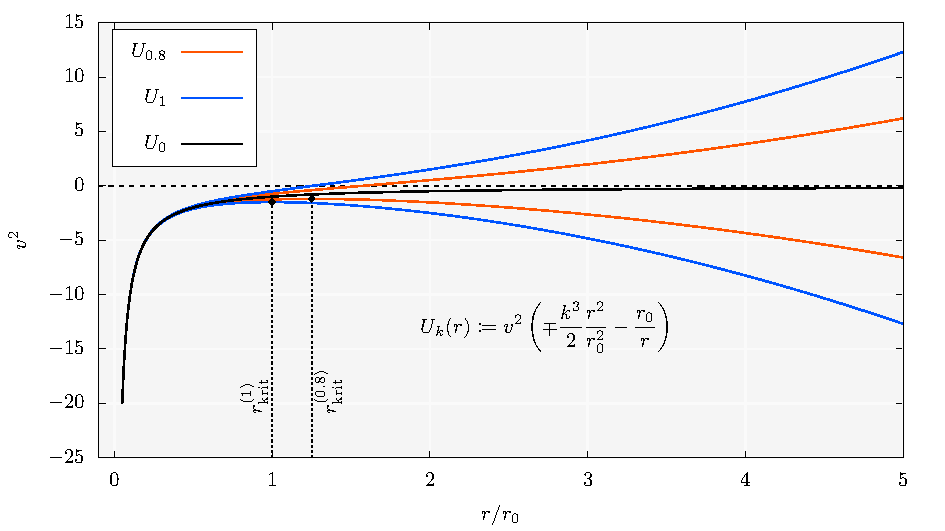
\includegraphics[width=0.95\textwidth]{exercise_1-plot.pdf}
          \caption{Die Abbildung zeigt das effektive Potential $U$ für verschiedene Werte von $k\define \frac{r_0}{r_\mathrm{krit}}$.}
        \end{figure}
      }
    \end{atiSubtaskSolutions}
  \end{atiSolution}
\end{document}